\chapter{Non-Uniform Meshes -- Results and Discussion} \label{cha:non-uniform-results-discussion}

\section{Results}

\subsection{Incompressible Navier-Stokes flow past a cylinder}

\begin{figure}
    \centering
    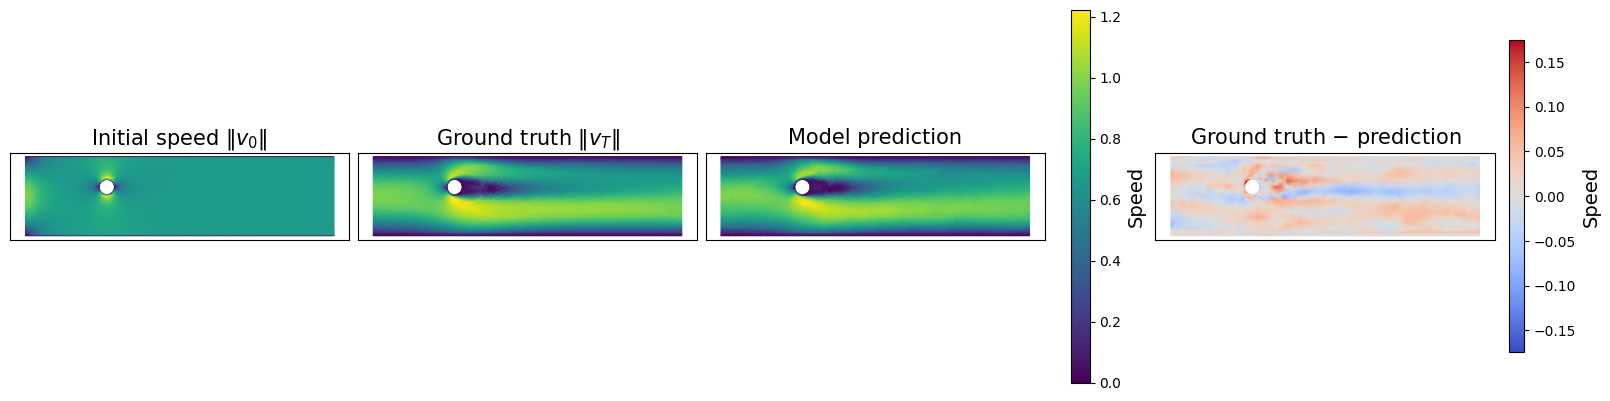
\includegraphics[width=0.99\textwidth]{figures/cylinder_flow_prediction_difference.png}
    \caption{\label{fig:geo-fno-cylinder-result}
    Representative Geo-FNO prediction on the cylinder flow dataset. The model predicts the horizontal and vertical velocity components separately; for visualization, the panels show the corresponding speed \(\|\mathbf{v}\|\). The panels show the initial speed field, the ground-truth final speed field, the model prediction, and the pointwise difference between prediction and ground truth on the irregular spatial mesh.}
\end{figure}

The Geo-FNO was first evaluated on the cylinder flow dataset. Figure~\ref{fig:geo-fno-cylinder-result} shows a representative prediction on a held-out test sample. Across the test set, the model reached an MSE of \(4.733\times10^{-3}\).

The prediction captures the main structure of the final velocity field, including the global flow pattern around the cylinder and the downstream wake. The difference plot shows that the error is not distributed uniformly across the domain. Larger errors occur primarily in regions where the velocity field changes more sharply, especially near the wake and around the obstacle. Despite these local errors, the qualitative agreement between the prediction and the ground truth indicates that Geo-FNO can learn the velocity-field mapping directly on the irregular point-cloud representation.

\subsection{HTGR column temperature dataset}

\begin{figure}
    \centering
    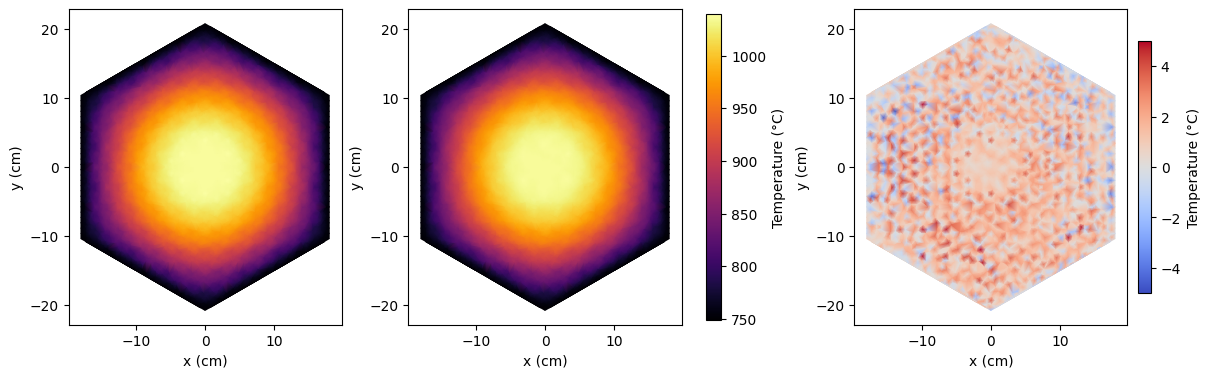
\includegraphics[width=1\textwidth]{figures/htgr_trigonometric_pred.png}
    \caption{\label{fig:geo-fno-htgr-result}
    Representative Geo-FNO prediction on the HTGR column temperature dataset. The panels show the ground-truth temperature field, the model prediction, and the signed difference between prediction and ground truth on the irregular spatial mesh. This sample corresponds to an axial level of \(z=30\,\mathrm{cm}\) and a boundary temperature of \(T=750\,^{\circ}\mathrm{C}\).}
\end{figure}

\begin{figure}
    \centering
    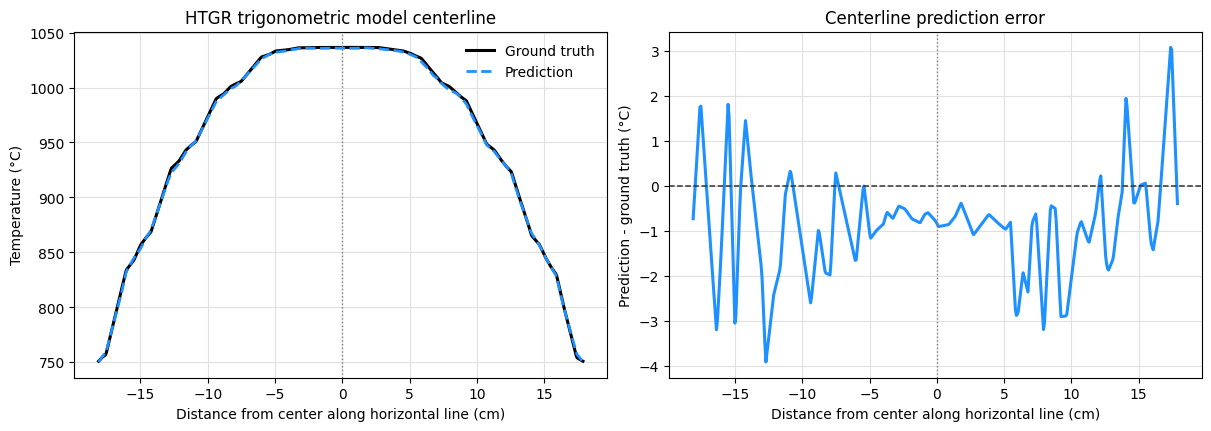
\includegraphics[width=0.9\textwidth]{figures/htgr_centerline.png}
    \caption{\label{fig:htgr-centerline}
    Horizontal centerline comparison for the HTGR sample shown in Figure~\ref{fig:geo-fno-htgr-result}. The left panel compares the ground-truth and predicted temperature profiles along the centerline, while the right panel shows the signed error \(T_{\mathrm{pred}}-T_{\mathrm{true}}\). The profile confirms that the model reproduces the temperature fall-off from the hot central region toward the cooler boundary, with remaining centerline errors of only a few degrees Celsius.}
\end{figure}

The Geo\hyp{}FNO was evaluated on the HTGR column temperature dataset described in Section~\ref{htgr-column-dataset}. Figure~\ref{fig:geo-fno-htgr-result} shows a representative prediction on a held\hyp{}out sample. Across the test set, the model reached an MSE of \(2.18\), corresponding to a relative RMSE of \(2.07\times10^{-3}\).

The predicted temperature field closely matches the ground truth. The dominant spatial temperature pattern is reproduced, with a hot central region and lower temperatures near the boundary. The difference plot shows local deviations of only a few degrees Celsius relative to an overall temperature range of several hundred degrees.

To examine whether the model reproduces the temperature fall-off from the center toward the boundary, a horizontal centerline profile was extracted from the same sample. Figure~\ref{fig:htgr-centerline} shows that the predicted and ground-truth profiles are nearly indistinguishable on the full temperature scale. The signed error remains within a few degrees Celsius along the profile, indicating that the apparent differences in the two-dimensional error plot are small local deviations rather than a substantial systematic error in the center-to-boundary temperature profile.




\section{Discussion}

\subsection{Incompressible Navier-Stokes Flow Past a Cylinder}

The cylinder flow dataset provides a challenging benchmark for mesh-free operator learning because the model must learn nontrivial fluid dynamics on a geometry that changes between samples. The cylinder radius and position vary across the dataset, and the solution is represented on a non-uniform point cloud rather than on a fixed Cartesian grid. The task is therefore not only to predict the velocity field, but also to do so across changing geometries and irregular sampling patterns.

Since the inlet speed and viscosity are fixed across the dataset, the Reynolds number varies directly with the cylinder radius,
\begin{equation}
Re = \frac{2UR}{\nu},
\end{equation}
where \(U\) is the inlet speed, \(R\) is the cylinder radius, and \(\nu\) is the kinematic viscosity \cite{cylinder-flow-re}. Larger cylinders therefore correspond to higher Reynolds numbers. For flow past a circular cylinder, periodic vortex shedding is expected above a critical Reynolds number of approximately \(Re\approx47\) \cite{cylinder-wake}, which provides a useful reference point for interpreting the prediction errors. Vortex shedding refers to the periodic formation and detachment of alternating vortices from opposite sides of the cylinder, resulting in oscillatory downstream wake behavior.

Figure~\ref{fig:cylinder-loss-re} shows the relative \(L^2\) velocity loss as a function of Reynolds number on the test set. The loss is elevated for the smallest cylinders, decreases for intermediate Reynolds numbers, and then increases gradually above the expected vortex-shedding onset. This suggests that the higher-\(Re\) samples are more difficult at least partly because the wake becomes increasingly unsteady. 

In this regime, the final state is not characterized only by a mean downstream wake shape, but also by the instantaneous position and phase of the wake structures. This makes the one-shot prediction task substantially harder. Vortex shedding does not begin immediately at the initial time of the prediction; the flow must first interact with the cylinder, the separated wake must develop, and the onset time and subsequent phase depend on the geometry and flow evolution. A model that maps directly from the initial state to the final state must therefore infer both the development of the oscillatory wake and its final phase without explicitly resolving the intermediate dynamics. Small errors in the inferred onset, frequency, or accumulated phase can place the wake displacement on the wrong side of the centerline, producing a large pointwise \(L^2\) error even when the predicted wake is qualitatively reasonable. This helps explain why the model tends to predict a smoother wake structure in the higher-\(Re\) cases.

\begin{figure}
    \centering
    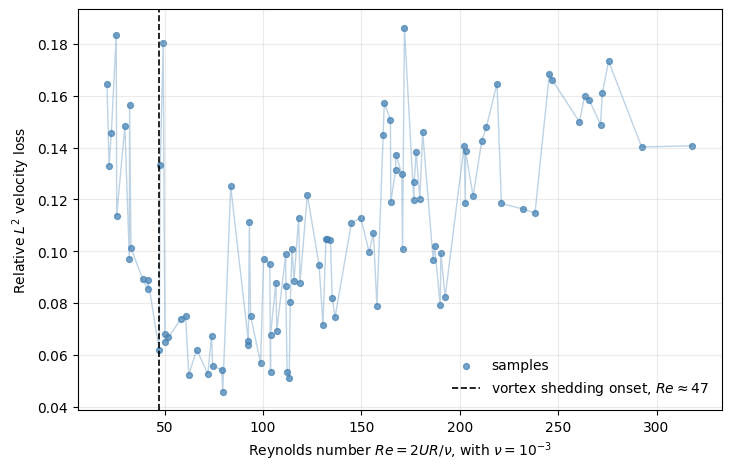
\includegraphics[width=0.8\textwidth]{figures/cylinder_flow_loss_vs_re.png}
    \caption{\label{fig:cylinder-loss-re}
    Relative \(L^2\) velocity loss for Geo-FNO on the cylinder flow test set as a function of Reynolds number \(Re=2UR/\nu\). Since \(U\) and \(\nu\) are fixed in the dataset, \(Re\) varies directly with the cylinder radius. The vertical dashed line marks the approximate onset of vortex shedding for flow past a circular cylinder, \(Re\approx47\).}
\end{figure}

This behavior is illustrated in Figure~\ref{fig:geo-fno-cylinder-result-unsteady}. The model captures the global flow around the cylinder and the approximate wake location, but the downstream wake in the prediction is smoother than in the ground truth. The resulting error is concentrated in the wake region, where small differences in the instantaneous wake structure are heavily penalized by the pointwise loss. This supports the interpretation that a significant part of the remaining error is associated with predicting detailed wake structure rather than with a failure to learn the dominant flow response.

\begin{figure}
    \centering
    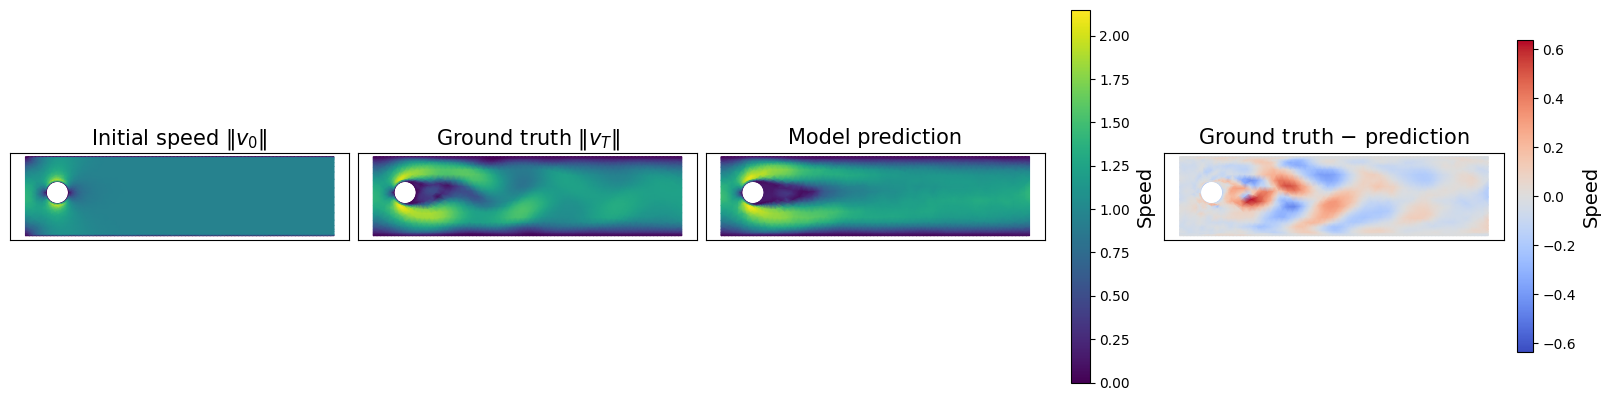
\includegraphics[width=0.99\textwidth]{figures/cylinder_flow_prediction_no_steady_state.png}
    \caption{\label{fig:geo-fno-cylinder-result-unsteady}
    Geo-FNO prediction on a cylinder flow sample with an oscillatory downstream wake. The model predicts the horizontal and vertical velocity components separately; for visualization, the panels show the corresponding speed \(\|\mathbf{v}\|\). The model captures the global flow structure but predicts a smoother wake than the ground truth, leading to larger localized errors downstream of the cylinder.}
\end{figure}

The elevated losses at the smallest Reynolds numbers are not explained by wake instability. These samples correspond to the smallest cylinders, where the obstacle boundary is represented by fewer mesh points and the near-cylinder disturbance occupies a smaller region of the point cloud. Small errors near the obstacle or in the immediate wake may therefore have a larger effect on the relative velocity loss. This remains a hypothesis, since no separate mesh-resolution diagnostic was performed for the small-radius cases.

Overall, Geo-FNO learns the dominant flow response across changing cylinder geometries, but the remaining errors concentrate in regimes where the final state is sensitive to small geometric or dynamical changes. The Reynolds-number trend points to wake instability as a major contributor at high \(Re\), while the small-radius errors may reflect the difficulty of representing very small obstacles on the irregular point cloud. The model can therefore learn the global flow response directly on a non-uniform mesh, but detailed one-shot prediction of sensitive wake structures remains challenging.

\subsection{HTGR Column Temperature Dataset}

The strong performance of Geo-FNO on the HTGR column temperature dataset should be interpreted in the context of the structure of the task. Compared to the cylinder flow benchmark, this problem is smoother and lower-dimensional. The output field is a scalar temperature distribution rather than a vector-valued velocity field, and the dominant physical behavior is governed by diffusion and heat transport rather than strongly nonlinear wake dynamics.

In addition, the spatial mesh is shared across all samples. Unlike the cylinder flow dataset, where both the geometry and the point cloud vary between samples, Geo-FNO is always evaluated on the same underlying irregular mesh. The model therefore does not need to adapt to changing geometries or different point distributions, and the challenge is focused primarily on learning the temperature field itself rather than learning across varying spatial representations.

The input space is also significantly simpler. As described in Section~\ref{htgr-column-dataset}, the prediction depends only on the boundary temperature and the axial position of the slice\footnote{As discussed in Appendix~\ref{appendix:htgr-input-engineering}, a trigonometric representation of \(z\) and \(T\) produced the lowest loss and was therefore used for the results reported here.}. This makes the task closer to learning a smooth parametric family of temperature fields than to solving a fully general operator learning problem with high-dimensional functional inputs.

Figure~\ref{fig:geo-fno-htgr-result} shows that Geo-FNO reproduces the dominant temperature structure accurately. The prediction captures the hot central region and the decrease toward the cooler boundary, while the difference plot shows only small local deviations relative to the overall temperature scale. To check whether the model reproduces the temperature fall-off from the center to the boundary, a horizontal centerline profile was extracted from the same sample. Figure~\ref{fig:htgr-centerline} shows that the predicted and ground-truth profiles are nearly indistinguishable on the full temperature scale. The signed error remains within a few degrees Celsius along the profile, indicating that the apparent differences in the two-dimensional error plot are small local deviations rather than a substantial systematic error in the center-to-boundary temperature profile.

These results show that Geo-FNO can be applied successfully to reactor-relevant temperature fields defined on non-uniform meshes without requiring interpolation onto a uniform Cartesian grid. This is useful in practice, since reactor geometries often involve curved boundaries and spatial layouts that are not naturally represented on regular grids.

At the same time, the relative simplicity of the HTGR task should be kept in mind. Because the geometry is fixed, the field is smooth, and the input space is low-dimensional, this experiment is best interpreted as a proof of applicability rather than a demonstration of performance on more complex reactor simulations. It shows that Geo-FNO can operate effectively on irregular reactor meshes, but does not by itself establish performance on fully general multiphysics reactor problems.

\subsection{Interpretation of Discretization Invariance on Mesh-Free Grids}

Section~\ref{mesh-free-discretization-invariance} explained that mesh-free discretization robustness requires comparing predictions for the same underlying physical sample across systematically varied point-cloud or mesh representations. The Geo-FNO experiments in this chapter do not provide such a controlled refinement study. Instead, they test whether Geo-FNO can learn directly on the irregular spatial representations available in the two datasets.

The cylinder flow dataset is the closer of the two to a mesh-free generalization test, because both the geometry and the point cloud vary between samples. However, these variations are coupled: changing the cylinder radius or position also changes the physical flow problem. As a result, the experiment tests generalization across geometries and irregular point clouds, but it does not isolate the effect of changing the discretization of one fixed physical sample.

The HTGR dataset has the opposite limitation. The spatial mesh is irregular, but it is shared across all samples. The experiment therefore shows that Geo-FNO can learn accurate temperature fields on a fixed irregular reactor mesh, but it does not test robustness to changes in mesh density, element size, or point placement.

The results should therefore be interpreted as evidence of applicability to irregular spatial representations rather than as a direct demonstration of mesh-free discretization invariance. A full test would require controlled families of meshes or point clouds for the same physical states, as discussed in Section~\ref{mesh-free-discretization-invariance}.